\documentclass[tikz,border=2pt]{standalone}
\usepackage{amsmath}
\usepackage{pgfplots}
\pgfplotsset{compat=1.18}

\begin{document}
% Γ(x) on (0,5] interpolates the factorials: Γ(n) = (n-1)! at the integers.
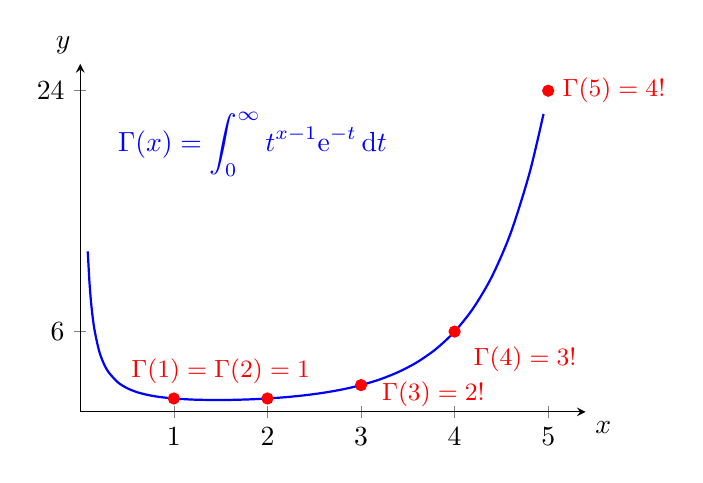
\begin{tikzpicture}
	\begin{axis}[
		axis lines=middle,
		xmin=0, xmax=5.4,
		ymin=0, ymax=26,
		xtick={1,2,3,4,5}, ytick={6,24},
		xlabel={$x$}, ylabel={$y$},
		xlabel style={below right}, ylabel style={above left},
		samples=160, smooth, clip=false,
		width=8cm, height=6cm
		]
		\addplot[thick, blue] coordinates {(0.08,11.9966) (0.1,9.5135) (0.12,7.8633) (0.15,6.2203) (0.2,4.5908) (0.25,3.6256) (0.3,2.9916) (0.4,2.2182) (0.5,1.7725) (0.6,1.4892) (0.7,1.2981) (0.8,1.1642) (0.9,1.0686) (1.0,1.0) (1.2,0.9182) (1.4,0.8873) (1.46,0.8856) (1.6,0.8935) (1.8,0.9314) (2.0,1.0) (2.2,1.1018) (2.4,1.2422) (2.6,1.4296) (2.8,1.6765) (3.0,2.0) (3.2,2.424) (3.4,2.9812) (3.6,3.717) (3.8,4.6942) (4.0,6.0) (4.2,7.7567) (4.4,10.1361) (4.6,13.3813) (4.8,17.8379) (4.95,22.2652)};
		\addplot[only marks, mark=*, red] coordinates {(1,1) (2,1) (3,2) (4,6) (5,24)};
		\node[red, anchor=west, font=\small] at (axis cs:5.05,24) {$\Gamma(5)=4!$};
		\node[red, anchor=north west, font=\small] at (axis cs:4.1,5.6) {$\Gamma(4)=3!$};
		\node[red, anchor=west, font=\small] at (axis cs:3.12,1.3) {$\Gamma(3)=2!$};
		\node[red, anchor=south, font=\small] at (axis cs:1.5,1.4) {$\Gamma(1)=\Gamma(2)=1$};
		\node[blue, anchor=west] at (axis cs:0.3,20) {$\Gamma(x)=\displaystyle\int_0^\infty t^{x-1}\mathrm{e}^{-t}\,\mathrm{d}t$};
	\end{axis}
\end{tikzpicture}
\end{document}
